\subsection{\texorpdfstring{$\tauTau$ channel}{tau-tau channel}}
\label{sect:tauTauCuts}
%In the context of MSSM, supersymmetric objects are produced in pairs to conserve R-parity quantum number. Therefore in the production of charginos from proton-proton collisions, one may consider the following interaction $$pp\rightarrow\PSGcpDo\PSGcmDo\rightarrow\sTau^{+}\nu_\tau \sTau^{-}\nu_\tau\rightarrow\tau^{+}\PSGczDo\nu_\tau\tau^{-}\PSGczDo\nu_\tau\rightarrow\tau^{+}\tau^{-} + 2\,\PSGczDo + 2\,\nu_\tau.$$ In the detector, what can be observed are only 2 tau leptons plus missing transverse energy from the presence of neutrinos and neutralinos in the final state.\\
%The tau leptons can decay leptonically, in 35\% of the time, or can decay via hadrons, which is occurring with 65\% of probability. Since there are two leptons in the final state, then the probability of having $\PSGcpDo\PSGcmDo \rightarrow \hadtau+e/\mu+\MET$ is about 46\%, while the probability of occurring $\PSGcpDo\PSGcmDo \rightarrow \hadtau+\hadtau+\MET$ is about 42\%. Hereafter, final states containing a lepton are referred to as $\leptonTau$ channel and those events where the two taus decays via hadrons are referred to as $\tauTau$. This section describes the cuts to enhance $\tauTau$ events. The list of cuts to select the $\leptonTau$ events can be found in Section~\ref{sect:leptonTauCuts}.\\    
In the final state with 2 hadronic taus, events are required to pass the following list of cuts
\begin{itemize}
\item \textbf{2 $\boldsymbol\tau_h$ Selection} At least two reconstructed opposite-sign tau objects, 
with $\pt>45\GeV$ and $|\eta|<2.1$, are required. Since the online trigger cuts require two taus with 
$\pt>35\GeV$, there is an offline cut on $\pt>45\GeV$ to get closer to the plateau of the trigger efficiency. 
Both taus not only are required to pass \emph{MediumCombinedIsoDBSumPtCorr3Hits} isolation requirement, 
but also should pass the Loose working point of the MVA3 anti-e discriminator, being \emph{LooseElectronMVA3Rejection}, 
as well as the Loose working point of the Muon2 anti-$\mu$ discriminator, being \emph{LooseMuon2Rejection}. 
In order to reject low mass QCD resonances, the invariant mass of two taus is required to be above 15 GeV. 
\item \textbf{$\boldsymbol e$ and $\boldsymbol\mu$ Veto} Extra electrons and muons are vetoed. This 
cut would help to reject backgrounds from di-boson events. Electron and muon rejection 
are exactly the same as in $\mu\Tau$ channel which is described in Sec.~\ref{sect:leptonTauCuts}.
\item \textbf{Z Veto} Events under the reconstructed Z mass peak are rejected, namely $|m_{\tau\tau}-m_{\Z}^{\rm rec}|>15\GeV$. 
In the reconstructed $\Z\rightarrow \Tau\Tau$ events passing above-mentioned set of cuts, events under the Z mass peak are fitted 
with a Gaussian function. The mean value of the fit is found to be about 70 GeV. Hence the invariant mass of two taus, $m_{\tau\tau}$, should be 
either below 55 GeV or above 85 GeV.  
\item \textbf{$\boldsymbol\mindphifour > $ 1} This cut is introduced against multi-jet events.  
\item \textbf{$\boldsymbol\mttwo>40\GeV$} Since SM background events with low \MET or fake \MET arising from miss-measured reconstructed object
 contribute to the lower values of $\mttwo$, then a moderate cut on this variable would improve data over MC ratio.  
\end{itemize}
After applying pre-selection cuts, two extra set of cuts are introduced, where each of them is sensitive to some regions of $\chione\PSGczDo$ mass plane: one aims the regions with large mass difference between charginos and neutralinos, the other one is dedicated for low mass-difference regions. It should be noted that the two search bins are chosen to be exclusive in order to be able to combine the statistics at the end.
\begin{itemize}
\item \textbf{Search \binone: sensitive to high $\boldsymbol\Delta m$}
A first set of cuts includes a cut on $\mttwo$.
\begin{itemize}
\item $\mttwo>90\GeV$.
\end{itemize}
\item \textbf{Search \bintwo: sensitive to low $\boldsymbol\Delta m$}
A second set of cuts includes some cuts on different variables listed below.
\begin{itemize}
\item bjets tagged with CSVM algorithm are vetoed.
\item $\mttwo<90\GeV$;
\item $\SumMT>250\GeV$;
\end{itemize}
\end{itemize}
The cut-flow-table can be found in table~\ref{tbl:cutflowtable}. The yields for three SUSY signal points, corresponding to a low mass difference $(m_{\chione}=180\GeV,m_{\PSGczDo}=60\GeV)$, a moderate mass difference $(m_{\chione}=240\GeV,m_{\PSGczDo}=40\GeV)$ and a high mass difference $(m_{\chione}=380\GeV,m_{\PSGczDo}=1\GeV)$, are presented in the table.   
\begin{sidewaystable}
%\begin{table}
\begin{center}
\begin{small}
\begin{tabular}{llccccccccccc}
\hline\hline
&  &SUSY(180,60)&(240,40)&(380,1)&Higgs&QCD&WW&W&DY&Top&Total Bkg&Data\\
\hline\hline
\multirow{5}{*}{Pre-Selection}&2 $\tau_h$ Selection&41.97&30.96&11.28&87.67&22081.57&13.71&595.80&2133.23&115.33&25027.32$\pm$6971.15&19615\\
&$e$ and $\mu$ Veto&38.68&27.89&9.87&81.53&19272.05&11.21&543.42&1961.29&95.85&21965.34$\pm$6387.87&18526\\
&Z Veo&37.80&26.28&9.21&70.50&18825.02&10.86&527.83&1333.37&88.53&20856.11$\pm$6383.93&17554\\
&$\mindphifour > $ 1&17.95&15.16&6.13&13.91&8426.98&3.66&192.11&276.27&13.67&8926.59$\pm$4404.31&5105\\
&$M_{T2} > $ 40&9.50&11.66&5.60&0.89&135.29&1.11&31.93&13.17&5.26&187.65$\pm$135.47&131\\
\hline
\binone&$M_{T2} > $ 90&0.59&3.89&3.81&0.17&$<$135.29&0.02&$<$1.28&0.56&$<$0.47&0.75$\pm$0.08&1\\
\hline
\multirow{3}{*}{\bintwo}&b-jet veto&7.92 &9.33 &4.67 &0.75&135.20&0.96&29.13&11.15&0.78&177.98$\pm$135.36&115\\
&$M_{T2} < $ 90&7.42 &6.17 &1.51 &0.61&135.20&0.94&29.13&10.65&0.78&177.32$\pm$135.36&114\\
&$\Sigma M_T^{\tau_i} > $ 250&2.17&3.36  &1.08&0.07&$<$135.20&0.15&0.43&0.81&0.53&1.99$\pm$0.87&2\\
\hline\hline
\end{tabular}
\caption{Cut-flow-table for $\tauTau$ channel. The quoted uncertainties are only statistical. When the remaining events from MC are zero, the weight of the events is reported as the upper bound.}
\label{tbl:cutflowtable}
\end{small}
\end{center}
%\end{table}
\end{sidewaystable}
The distributions of $\mttwo$ and $\SumMT$ after applying pre-selection cuts are shown in figure~\ref{fig:comparison}. 
The b-jet veto cut is also applied on the $\SumMT$ distribution. For both plots, the shape of QCD MC events 
is taken from same-sign events, which means that same selection cuts as pre-selection are applied except for the charge 
requirement which is reversed. Then the distribution of QCD MC events are found from data after non-QCD MC subtraction 
in the same-sign region. It can be concluded that data and MC are in reasonable agreement within the statistical uncertainties. 
\begin{figure}[!Hhtb]
\centering
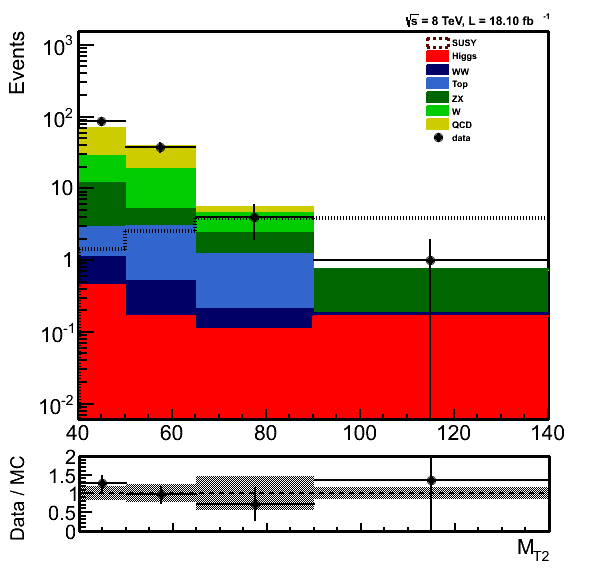
\includegraphics[angle=0,scale=0.35]{TauTauFigs/MT2_SSQCD_dataunblinding.png}
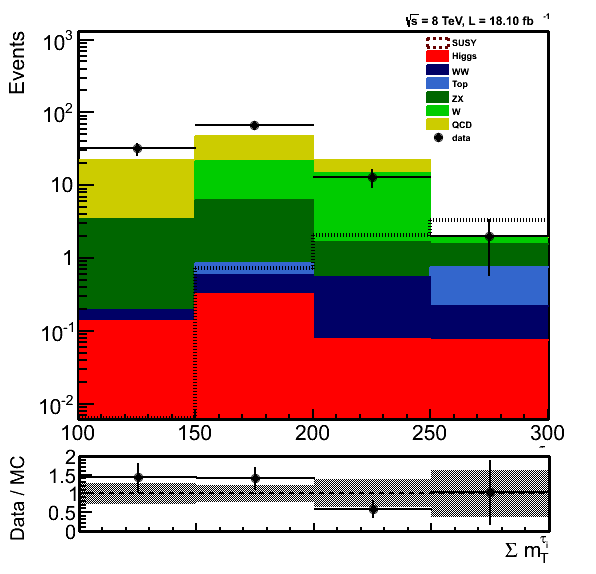
\includegraphics[angle=0,scale=0.35]{TauTauFigs/SumMT_SSQCD_dataunblinding.png} \\
\caption{The distributions of \mttwo (left) and \SumMT (right) after pre-selection. The b-jet veto cut is also applied on the right plot.}
\label{fig:comparison}
\end{figure}
